\chapter{Konwolucyjne sieci neuronowe}
Konwolucyjne sieci neuronowe (ang. Convolutional Neural Networks)
\section{Zarys historyczny}
\section{Przykłady współczesnych topologii}
\subsection{AlexNet}
Sieć AlexNet, której nazwa pochodzi od imienia głównego twórcy tej architektury Alexa Krizhevsky, zawiera blisko 60 milionów parametrów i 650 tysięcy neuronów. Architekturę zaprezentowano na Rys. \ref{AlexNetTopology}
\begin{figure}[h!]
	\centering
	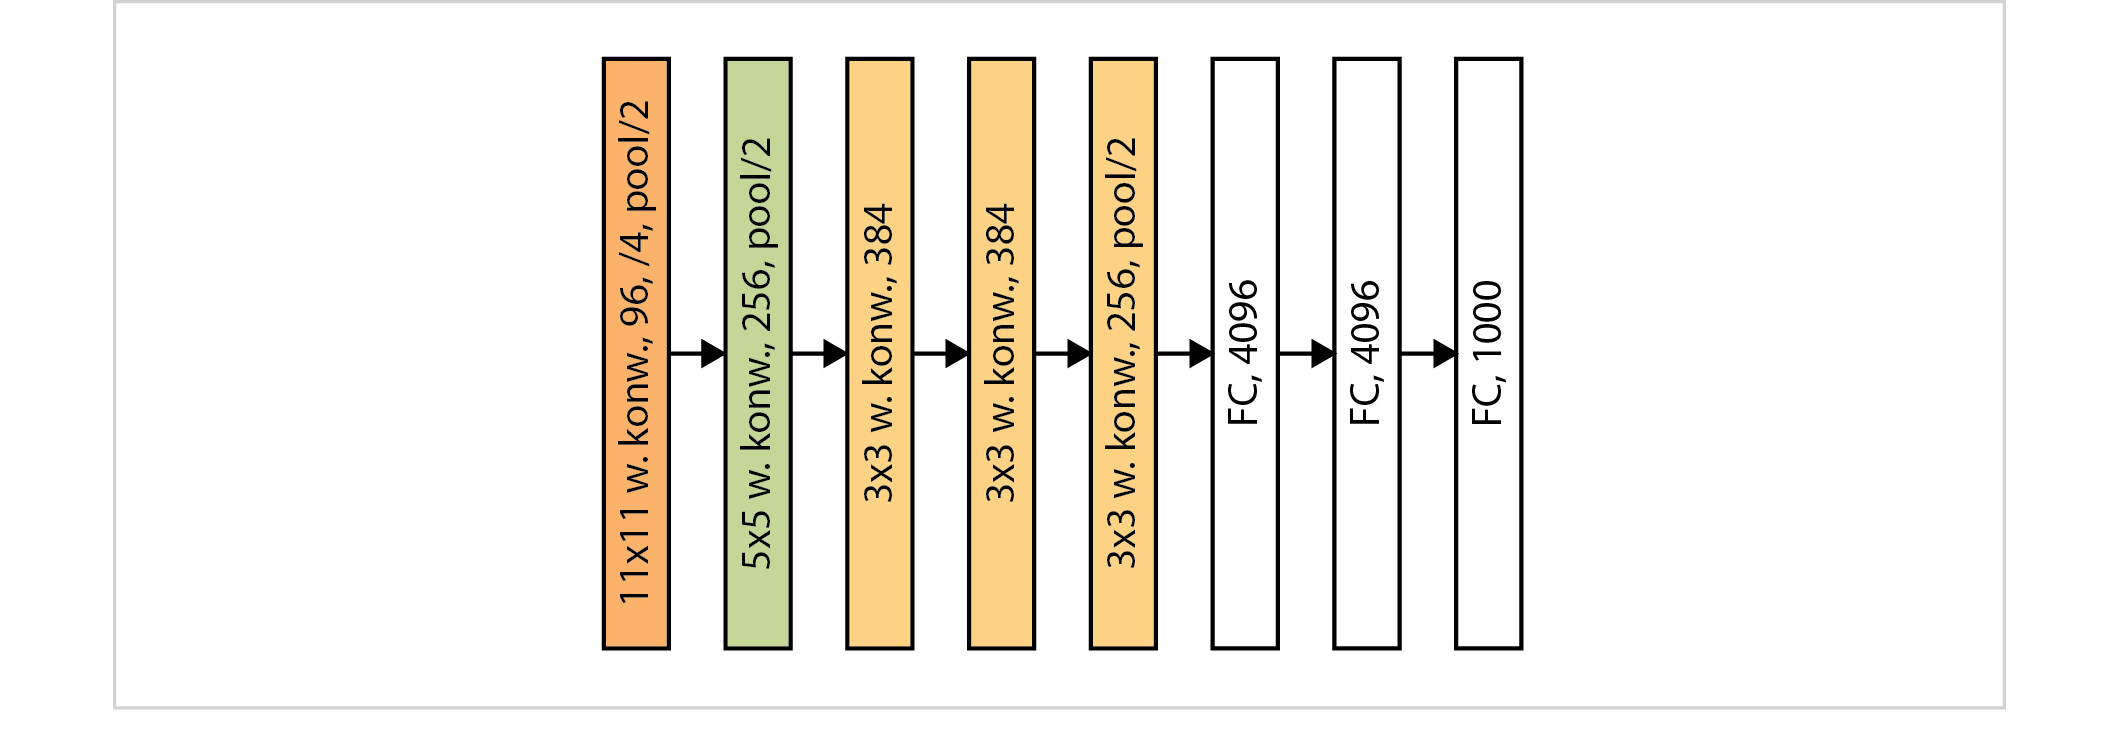
\includegraphics[width=0.55\textwidth]{figures/AlexNet.png}
	\caption{Topologia architektury AlexNet.}
	\label{AlexNetTopology}
\end{figure}

W skład topologii wchodzi pięć warstw konwolucyjnych i trzy typu fully-connected. Po pierwszej, drugiej i piątej warstwie konwolucyjnej występują operacje typu max-pool. 

Pierwsza warstwa konwolucyjna przyjmuje na wejściu dane o wymiarze 224$\times$224, na których wykonywana jest operacja splotu z 96 filtrami z maską o wymiarach 11$\times$11 i krokiem 4. Następnie wykonywana jest operacja max-pool na obszarze 2$\times$2. W wyniku tych operacji powstaje 96 obrazów (cech) o wymiarach 27$\times$27.


\subsection{GoogleNet}
\subsection{ResNet}
\subsection{Złożenia}
\section{Zastosowania w medycynie}
\section{Problem nadmiernego dopasowania}
\section{Problem redukcji wymiarowości}